\documentclass[]{book}

%These tell TeX which packages to use.
\usepackage{array,epsfig}
\usepackage{amsmath}
\usepackage{amsfonts}
\usepackage{amssymb}
\usepackage{amsxtra}
\usepackage{amsthm}
\usepackage{mathrsfs}
\usepackage{color}
\usepackage{graphicx}
\usepackage{bm}
\usepackage{tikz}
%\usepackage{widthof}
\usetikzlibrary{arrows}

%Here I define some theorem styles and shortcut commands for symbols I use often
\theoremstyle{definition}
\newtheorem{defn}{Definition}
\newtheorem{thm}{Theorem}
\newtheorem{cor}{Corollary}
\newtheorem*{rmk}{Remark}
\newtheorem{lem}{Lemma}
\newtheorem*{joke}{Joke}
\newtheorem{ex}{Example}
\newtheorem*{soln}{Solution}
\newtheorem{prop}{Proposition}

\newcommand{\lra}{\longrightarrow}
\newcommand{\ra}{\rightarrow}
\newcommand{\surj}{\twoheadrightarrow}
\newcommand{\graph}{\mathrm{graph}}
\newcommand{\bb}[1]{\mathbb{#1}}
\newcommand{\Z}{\bb{Z}}
\newcommand{\Q}{\bb{Q}}
\newcommand{\R}{\bb{R}}
\newcommand{\C}{\bb{C}}
\newcommand{\N}{\bb{N}}
\newcommand{\M}{\mathbf{M}}
\newcommand{\m}{\mathbf{m}}
\newcommand{\MM}{\mathscr{M}}
\newcommand{\HH}{\mathscr{H}}
\newcommand{\Om}{\Omega}
\newcommand{\Ho}{\in\HH(\Om)}
\newcommand{\bd}{\partial}
\newcommand{\del}{\partial}
\newcommand{\bardel}{\overline\partial}
\newcommand{\textdf}[1]{\textbf{\textsf{#1}}\index{#1}}
\newcommand{\img}{\mathrm{img}}
\newcommand{\ip}[2]{\left\langle{#1},{#2}\right\rangle}
\newcommand{\inter}[1]{\mathrm{int}{#1}}
\newcommand{\exter}[1]{\mathrm{ext}{#1}}
\newcommand{\cl}[1]{\mathrm{cl}{#1}}
\newcommand{\ds}{\displaystyle}
\newcommand{\vol}{\mathrm{vol}}
\newcommand{\cnt}{\mathrm{ct}}
\newcommand{\osc}{\mathrm{osc}}
\newcommand{\LL}{\mathbf{L}}
\newcommand{\x}{\bm{x}}
\newcommand{\UU}{\mathbf{U}}
\newcommand{\support}{\mathrm{support}}
\newcommand{\AND}{\;\wedge\;}
\newcommand{\OR}{\;\vee\;}
\newcommand{\Oset}{\varnothing}
\newcommand{\st}{\ni}
\newcommand{\wh}{\widehat}

%Pagination stuff.
\setlength{\topmargin}{-.3 in}
\setlength{\oddsidemargin}{0in}
\setlength{\evensidemargin}{0in}
\setlength{\textheight}{9.in}
\setlength{\textwidth}{6.5in}
\pagestyle{empty}



\begin{document}


\begin{center}
{\Large The gambler's ruin \hspace{0.5cm} Part 1 (two-player)}\\
\textbf{Alireza Abrehforoush}\\ %You should put your name here
Date: 6/29/2022 %You should write the date here.
\end{center}

\vspace{0.2 cm}


\section*{Recursion}
\subsection*{Model}
Consider $n$ agents on a ring, labeled by $1,\ldots, n$. 
Each agent plays either of the strategies $A$ or $B$ over time $t=0,1,\ldots$.
At each time $t$, a single agent becomes active to update its strategy: If its strategy is different from those of its neighbors, she is \emph{equilibrium}; otherwise, she switches.
The activation of the agents follows a stochastic process, determined by the i.i.d. multinomial random variables $I_0,I_1,\ldots\in\{1,\ldots,n\}$ with mean $p$, where $I_t$ is the active agent at time $t$.
We are interested in finding the expected time until the network reaches an equilibrium. 
Stack all agents' configuration into the vector $\x = [x_1,\ldots,x_n]$ where $x_i$ denotes the strategy of agent $i$.
\begin{figure}[ht]
    \centering
    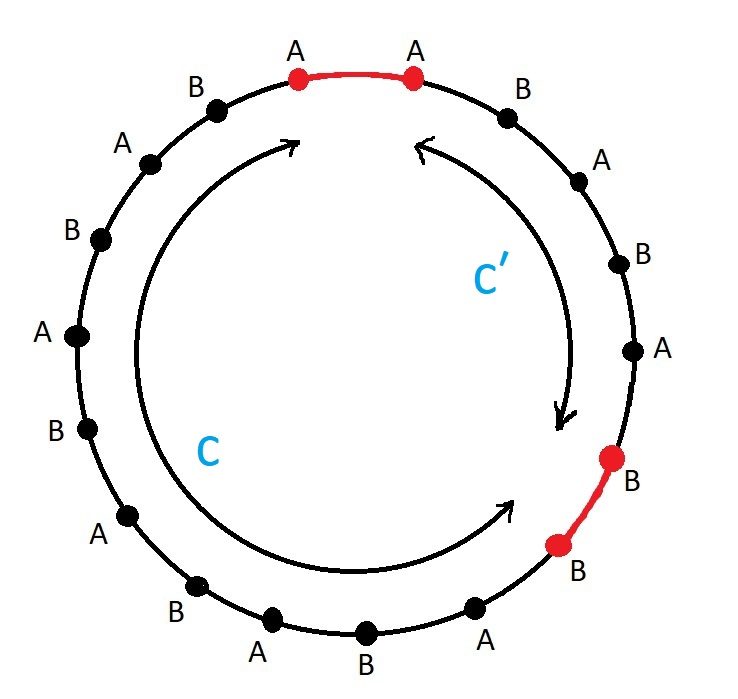
\includegraphics[width=0.4\textwidth]{model1.jpg}
    \caption{two-player with $n=18$ and initial value of $c$ and $c^{\prime}$ for players}
    \label{fig:mesh1}
\end{figure}

\subsection*{Equivalent representation}
The problem can be interpreted as follows. 
Color red every adjacent pairs of same-strategy agents on the ring. 
We also color red the arc between every such pair. 
At each time step, if any of the non-red agents become active, they do not switch. 
If any of the red agents who are adjacent to a non-red agent become active, they switch strategies, causing the red arc to move one unit to clockwise or counterclockwise. 
If a red agent who is adjacent with two other red agents becomes active, then both red arcs become black. 

Case 1: First, we consider initial configurations $\x(0)$, where there exists exactly two non-adjacent pairs of adjacent same strategy-playing agents. 
Equivalently, there are two non-adjacent red arcs in the ring, labeled by 1 and 2.
%Correspondingly, the right of each arc is the counter clockwise direction...
Let \emph{state $c$} and \emph{$c^{\prime}$} denote the number of continuous arcs between the arc 1 and arc 2.
Clearly, $c, c^{\prime} \in\{0,\ldots,n\}$.

\subsection*{Recursive equation}
%%%%%%%%%%%%%%%%%%%%%%%%%%%%%%%%%%%
%Define the \textdf{$\ell^1$-norm} on $\R^n$ by
%	$$\|x\|_1 = \sum_{i=1}^n |x^i|,$$
%	and define the \textdf{sup-norm} on $\R^n$ by
%	$$\|x\|_\infty = \sup\left\{|x^i|\right\}.$$
%	Show that these satisfy Theorem~1.
%%%%%%%%%%%%%%%%%%%%%%%%%%%%%%%%%%%
\subsubsection*{Model}
We model the problem through the following Markov chain.
%graph
\begin{center}
\begin{tikzpicture}
\tikzset{vertex/.style = {shape=circle,draw,minimum size=3em}}
\tikzset{edge/.style = {->,> = latex'}}
% vertices
\node[vertex] (a) at  (-4,0) {$0$};
\node[vertex] (b) at  (1,3) {$n-1$};
\node[vertex] (c) at  (6,0) {$n-2$};
\node[vertex] (d) at  (1,-3) {$n$};
\node[vertex] (a1) at (-2,0) {$1$};
\node[vertex] (a2) at (0,0) {$2$};
%edges
\draw[->] (a) edge  [loop above] node {$1-3p$} ();
\draw[->] (b) edge  [loop above] node {$1$} ();
\draw[->] (c) edge  [loop above] node {$1-3p$} ();
\draw[->] (d) edge  [loop above] node {$1$} ();
\draw[->] (a1) edge  [loop above] node {$1-4p$} ();
\draw[->] (a2) edge  [loop above] node {$1-4p$} ();

\path[->] (a) edge[bend right]      node[above]{$p$} (d);
\path[->] (c) edge[bend left]      node[above]{$p$} (d);

\path[->] (a) edge[bend left]     node[above]                      {2p} (a1);
\path[->] (a1) edge[bend left]     node[above]                      {2p} (a);

\path[->] (a1) edge[bend left]     node[above]                      {2p} (a2);
\path[->] (a2) edge[bend left]     node[above]                      {2p} (a1);

\path (a2) to node {\dots} (c);
\node [shape=circle,minimum size=1.5em] (a3) at (2,0) {};
\path[->] (a2) edge[bend left]     node[above]                      {2p} (a3);
\path[->] (a3) edge[bend left]     node[above]                      {2p} (a2);

\node [shape=circle,minimum size=1.5em] (c1) at (4,0) {};
\path[->] (c) edge[bend left]     node[above]                      {2p} (c1);
\path[->] (c1) edge[bend left]     node[above]                      {2p} (c);
\end{tikzpicture}
\end{center}
%graph

We consider states $0,1,\ldots,n$ corresponding to the configuration with $c = i \in \left\{0,1,\ldots,n\right\}$. 
Let $t_c$ denote the expected equilibrium time, starting from state $c$.
The changes in $c$ are governed by the following recursive equation:
\begin{equation}    \label{mainEquation}
    t_c 
    = 2p t_{c-1}  + 2p t_{c+1} + (1 - 4p)t_{c} + 1\\
    = \frac{1}{2}t_{c-1} + \frac{1}{2}t_{c+1} + \frac{1}{4p}, \quad c = 1,\ldots,n-3,
\end{equation}

\begin{equation}\label{recursiveEquation_t_0}
    t_0 = pt_{n} + 2pt_1 + (1-3p)t_0  + 1 = \frac{2}{3}t_1 + \frac{1}{3p}, \qquad t_{n-2}=t_0, \qquad t_n = 0;
\end{equation}





\subsubsection*{Initial conditions}

From (1) and (2) we can infer
\begin{multline*}
    \\
    t_1 = \frac{1}{2}t_0 + \frac{1}{2}t_2 + \frac{1}{4p}\\
    t_2 = \frac{1}{2}t_1 + \frac{1}{2}t_3 + \frac{1}{4p}\\
    t_3 = \frac{1}{2}t_2 + \frac{1}{2}t_4 + \frac{1}{4p}\\
    \vdots\\
    t_{n-3} = \frac{1}{2}t_{n-4} + \frac{1}{2}t_{n-2} + \frac{1}{4p}\\
    \sum_{i=1}^{n-3} t_i = \frac{1}{2}\left[ \sum_{i=0}^{n-4} t_i + \sum_{i=2}^{n-2} t_i \right] + \frac{n-3}{4p} \Rightarrow t_1 + t_{n-3} = \frac{1}{2}\left(t_0 + t_1 + t_{n-3} + t_{n-2}\right) + \frac{n-3}{4p}\\
    \Rightarrow \frac{1}{2}\left(t_1 + t_{n-3}\right) = \frac{1}{2}\left(t_0 + t_{n-2}\right) + \frac{n-3}{4p}\\
    \qedsymbol
\end{multline*}
as pairs of $c$ and $c^{\prime}$ for which the equation $c + c^{\prime} = n - 2$ holds correspond to same configurations we have $t_{1} = t_{n-3}$ and $t_{0} = t_{n-2}$. so
\begin{equation}
    t_1 = t_0 + \frac{n-3}{4p}
\end{equation}



From (2) and (3) we can infer

\begin{center}
\begin{equation} \label{temp9}
    t_1 = \frac{2}{3}t_1 + \frac{1}{3p} + \frac{n-3}{4p} \Rightarrow t_1 = \frac{1}{p} + \frac{3n-9}{4p} = \frac{3n-5}{4p}
\end{equation}
\begin{equation} \label{temp10}
    t_0 = t_1 - \frac{n-3}{4p} = \frac{2n-2}{4p}
\end{equation}
\end{center}


\subsubsection*{Solution}
\qquad
We now have a non-homogeneous linear recurrence relation with (1) as relation and (4) and (5) as initial conditions. The solution ($t_c$)
of a non-homogeneous recurrence relation has two parts.
First part is the solution ($t^{(h)}_{c}$)
of the associated homogeneous recurrence relation and the second part is the particular solution ($t^{(p)}_{c}$).
$$
        t_c = t^{(h)}_{c} + t^{(p)}_{c}
$$
First we rewrite (1) in standard form.
\begin{equation}
    t_{c+1} = 2t_c - t_{c-1} - \frac{1}{2p}
\end{equation}
The characteristic polynomial corresponding to the homogeneous part is as follows:
$$
r^2 - 2r + 1 = 0 \Rightarrow r = 1
$$
Thus the general solution is of the form
$$
t_c = \alpha_{1}c 1^c + \alpha_{2} 1^c
$$
Armed with that knowledge, and since the non-homogeneous part is also a polynomial (in this case of degree zero) which is itself a degenerate case of being of the form $1^c$ as well, we multiply by $c$ enough times to make it distinct from the other already known parts. I.e. we expect the non-homogeneous part to be of the form $\beta c^2$. Plugging this into the recurrence, we have:
$$
\beta (c+1)^2 = 2\beta c^2 - \beta (c-1)^2 - \frac{1}{2p} \Rightarrow \beta = -\frac{1}{4p}
$$
So, we expect
$$
t_c = \alpha_1 c + \alpha_2 - \beta c^2 = \alpha_1 c + \alpha_2 -\frac{1}{4p}c^2
$$
using initial conditions we have:
$$
t_0 = \alpha_1 \times 0 + \alpha_2 - \frac{1}{4p}\times 0 = \frac{2n-2}{4p} \\
\Rightarrow \alpha_2 = \frac{2n-2}{4p}
$$
and
$$
t_1 = \alpha_1 + \frac{2n-2}{4p} -\frac{1}{4p} = \frac{3n-5}{4p} \Rightarrow \alpha_1 = \frac{n-2}{4p}
$$
Thus, the final closed form is:
\begin{equation} \label{closed form}
    t_c = \frac{(n-c)(c+2) - 2}{4p}\\
\end{equation}


\begin{figure}[ht]
    \centering
    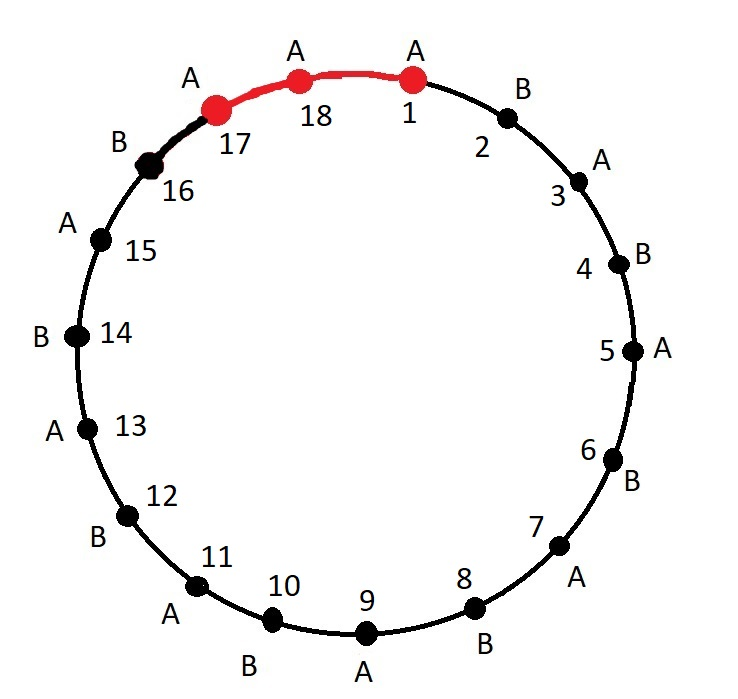
\includegraphics[width=0.4\textwidth]{figures/t0.jpg}
    \caption{configuration with $c = 0$}
    \label{fig:mesh2}
\end{figure}


% \begin{align*}
%     t_{0} 
%     &= \frac{1}{p} t_{c-1} + pt_{c+1} + 1... \\
%     &= \frac{1}{p} t_{c-1} + pt_{c+1} + 1... 
% \end{align*}

% \begin{figure}[h]
%     \centering
%     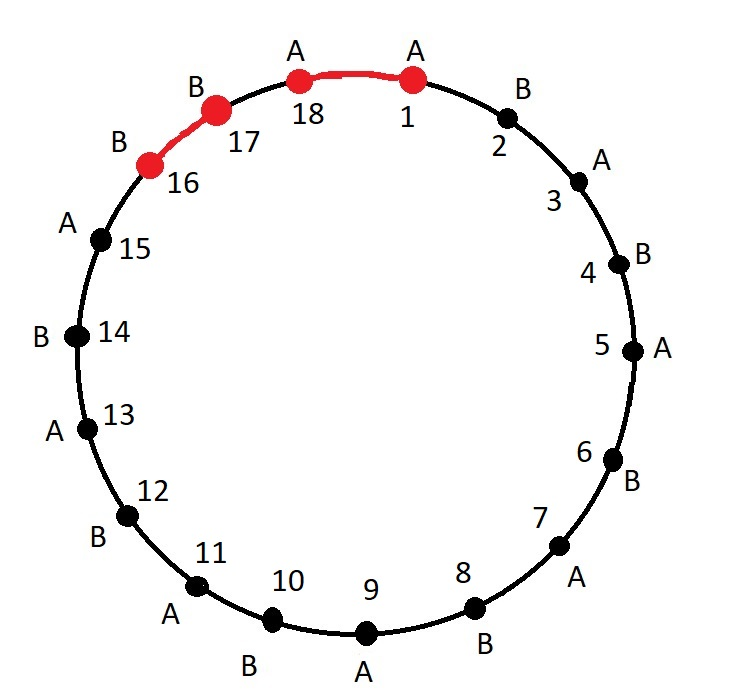
\includegraphics[width=0.4\textwidth]{t1.jpg}
%     \caption{configuration with $c = 1$}
%     \label{fig:mesh1}
% \end{figure}

% \begin{equation*}
%     \begin{cases}
%       t_{0} = t_{n-2} = p(1) + 2p(t_{1}+1)  \\
%     \end{cases}.
% \end{equation*}
% To solve the equation, for $c = 1,\ldots,n-1$, we obtain
% \begin{align*}
%      t_{c+1} 
%     &= \frac{1}{p} t_{c-1} + pt_{c+1} + 1... \\
%     &= \frac{1}{p} t_{c-1} + pt_{c+1} + 1... 
% \end{align*}
% $$t_{a} = \frac{1}{2}t_{a-1} + \frac{1}{2}t_{a+1} + 1 \newline$$

% $$
% \Rightarrow t_{a+1} = 2t_{a} - t_{a-1} - 2 \newline
% $$

% $$
% \Rightarrow t_{a} = 2t_{a-1} - t_{a-2} - 2
% $$
	
% \subsection*{Initial values}
% \subsubsection*{mine}


% \subsubsection*{yours}
% $$
% \begin{cases}
%   t_{0} = 0 + \frac{2}{k}t_{1} + 1 \\
%   X_{k} = 0
% \end{cases}
% $$

% \subsection*{Solving recurrence}
% \subsubsection*{mine}
% $$
% r^2 -2r + 1 = 0 \newline
% $$
% $$
% \Rightarrow t^{(h)}_{a} = \alpha_{1} + \alpha_{2}n
% $$

% \subsubsection*{yours}
% $$
% -2\alpha^2 + \alpha + 2 = 0 \newline
% $$
% $$
% \Rightarrow \alpha = \frac{-1\pm \sqrt{1+16}}{-4} \newline
% $$



% \begin{proof}
% 	% WRITE YOUR PROOF HERE.
% \end{proof}





\end{document}


